\chapter{Experimental Setup and Empirical Evaluation}
\label{ch:experiments}

\begin{chapterabstract}
This chapter defines the evaluation protocol and reports the empirical
behaviour of the proposed scheduler. It specifies the video environment and
parameters, formalises the metrics --- chief among them Semantic Compute
Efficiency --- describes the baseline policies, presents a preliminary
single-video measurement of the proposed three-tier scheduler, and outlines
the comparative and ablation studies that complete the evaluation. The
proposed-scheduler figures reported here are measured; the baseline rows of
the comparison are runs in progress and are explicitly marked as such.
\end{chapterabstract}

\section{Video Environment and Parameters}
\label{sec:exp-setup}

Evaluation uses continuous video streams representative of edge robotic
operation, containing extended quiescent intervals interspersed with bursts of
genuine semantic change (objects entering and leaving view, agents being
replaced, and reconfiguration of the observed workspace). The preliminary
measurement reported in Section~\ref{sec:exp-results} was obtained on a single
long stream of $56{,}314$ frames (approximately $2$~hours $16$~minutes of
video) processed end-to-end. All policies process the same frames through
identical detection, tracking, and embedding stages, so observed differences
arise solely from the allocation decision. Unless stated otherwise, runs use
the default configuration of Table~\ref{tab:hyperparams} on the hardware of
Section~\ref{sec:arch-hardware}.

\section{Formal Evaluation Metrics}
\label{sec:exp-metrics}

For every run the following quantities are recorded:

\begin{itemize}
  \item \textbf{VLM call rate} --- the fraction of frames on which the VLM is
  invoked (Tier 2 or 3); the primary measure of compute saved.
  \item \textbf{Cache hit rate} --- the fraction of frames served from the
  semantic cache (Tier 1) without any VLM invocation.
  \item \textbf{Average latency} (ms/frame) --- mean wall-clock time per frame,
  including the monitor and any invoked reasoning.
  \item \textbf{Throughput} (FPS) --- frames processed per second.
  \item \textbf{Semantic retention} --- mean similarity between the delivered
  output and the every-frame oracle output, in $[0,1]$.
  \item \textbf{Semantic Compute Efficiency (SCE)} --- retention divided by
  normalised compute cost, per Equation~(\ref{eq:sce}).
\end{itemize}

Semantic retention and SCE jointly capture the central trade-off: a policy
that saves compute by skipping reasoning is only valuable if the information
it delivers remains close to what exhaustive reasoning would have produced.

\section{Baseline Policies}
\label{sec:exp-baselines}

The proposed scheduler is compared against four baselines, each expressed as a
policy object (Section~\ref{sec:arch-controlflow}):

\begin{enumerate}
  \item \textbf{Every-frame} --- invokes the VLM on every frame. Defines the
  fidelity oracle (retention $=1$) and the compute reference (normalised cost
  $=1$, so $\mathrm{SCE}=1$ by construction).
  \item \textbf{Uniform sampling} --- invokes the VLM every $K$ frames
  irrespective of content ($K=30$, matching the \texttt{fixed\_interval}
  configuration used in the experiments), giving a call rate of $1/30 \approx
  0.033$ by construction.
  \item \textbf{Motion gating} --- invokes the VLM when frame-to-frame pixel
  motion exceeds a fixed threshold.
  \item \textbf{Embedding threshold} --- invokes the VLM when CLIP embedding
  drift alone exceeds a threshold ($D_{\text{embed}}$ only; the
  $\beta=\gamma=0$ special case of the proposed signal).
  \item \textbf{Proposed} --- the full fused-drift, three-tier scheduler.
\end{enumerate}

\section{Quantitative Performance Analysis}
\label{sec:exp-results}

Table~\ref{tab:proposed-results} reports the measured behaviour of the
proposed three-tier scheduler on the single long stream. Of the $56{,}314$
frames, $90.19\%$ were served from the semantic cache at Tier~1, $9.68\%$
triggered a lightweight Tier-2 query, and only $0.13\%$ ($73$ frames) required
full Tier-3 reasoning, yielding an overall VLM call rate of $9.81\%$ --- a
roughly tenfold reduction in reasoning invocations relative to an every-frame
policy. With semantic retention measured at $1.000$ on this stream, the
resulting Semantic Compute Efficiency is approximately $10$, consistent with
$\mathrm{SCE} \approx \text{retention} / \text{call rate} = 1.0/0.098$.

\begin{table}[htbp]
\centering
\caption[Measured proposed-scheduler performance]{Measured performance of the
proposed three-tier scheduler on a single continuous stream of $56{,}314$
frames ($\approx 2$\,h\,$16$\,m).}
\label{tab:proposed-results}
\small
\begin{tabular}{@{}lr@{}}
\toprule
\textbf{Quantity} & \textbf{Value} \\
\midrule
Total frames processed        & $56{,}314$ \\
Stream duration               & $8{,}185.8$\,s \\
VLM calls (Tier 2 + Tier 3)   & $5{,}524$ \\
\quad Tier 1 (cache reuse)    & $50{,}790$ \;($90.19\%$) \\
\quad Tier 2 (lightweight)    & $5{,}451$ \;($9.68\%$) \\
\quad Tier 3 (full reasoning) & $73$ \;($0.13\%$) \\
VLM call rate                 & $0.098$ \\
Cache hit rate                & $0.902$ \\
Average latency               & $144.9$\,ms/frame \\
Throughput                    & $6.88$\,FPS \\
Average drift $\bar{D}_t$     & $0.103$ \\
Semantic retention            & $1.000$ \\
Semantic Compute Efficiency   & $\approx 10.0$ \\
\bottomrule
\end{tabular}
\end{table}

The very high cache hit rate and unit retention on this particular stream
reflect its composition: a single, largely stable scene with limited semantic
variation, in which long quiescent intervals dominate and the cached output
remains faithful to the every-frame reference for extended periods. This is
the regime in which semantic-aware scheduling is most advantageous, and the
result should be read as a favourable-case demonstration rather than a
worst-case bound; streams with denser semantic change will exhibit lower cache
hit rates and correspondingly lower (but still favourable) SCE.

Figure~\ref{fig:tiers} visualises the tier distribution of this run, making
explicit that the overwhelming majority of frames are resolved without any
reasoning. Figure~\ref{fig:drift} shows a representative segment of the
per-frame drift signal with the two decision thresholds: quiescent runs sit
well below $\tau_{\text{low}}$ and are served from cache, while occasional
semantic transitions cross $\tau_{\text{high}}$ and trigger full reasoning ---
the mechanism that produces the $73$ Tier-3 invocations.

\begin{figure}[htbp]
\centering
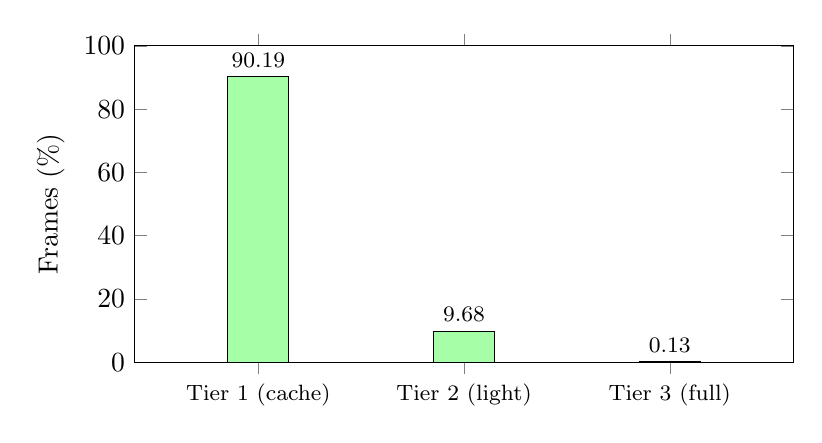
\begin{tikzpicture}
\begin{axis}[
  width=0.82\textwidth, height=5.6cm,
  ybar, bar width=22pt,
  ymin=0, ymax=100,
  ylabel={Frames (\%)},
  symbolic x coords={Tier 1 (cache), Tier 2 (light), Tier 3 (full)},
  xtick=data, x tick label style={font=\footnotesize},
  ylabel near ticks, nodes near coords, nodes near coords style={font=\footnotesize},
  enlarge x limits=0.3,
]
\addplot[fill=green!35] coordinates
  {(Tier 1 (cache),90.19) (Tier 2 (light),9.68) (Tier 3 (full),0.13)};
\end{axis}
\end{tikzpicture}
\caption[Tier distribution of the proposed run]{Measured tier distribution of
the proposed scheduler over $56{,}314$ frames. Over $90\%$ of frames are
resolved from cache with no VLM invocation.}
\label{fig:tiers}
\end{figure}

\begin{figure}[htbp]
\centering
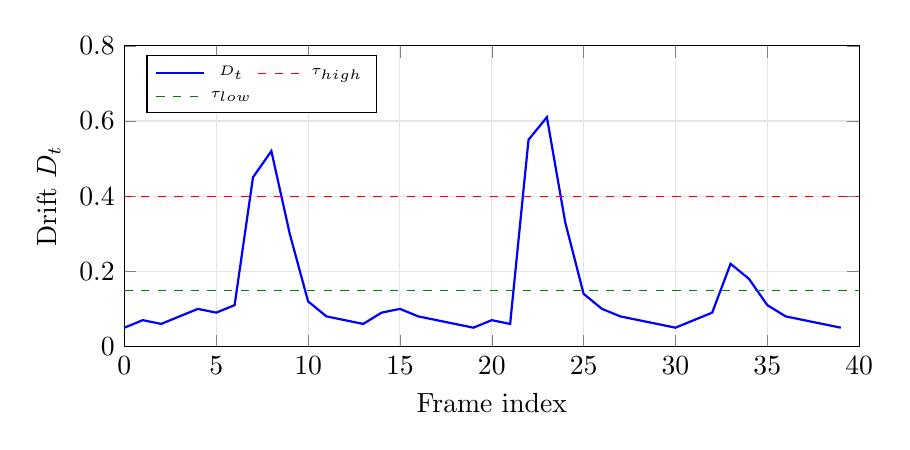
\begin{tikzpicture}
\begin{axis}[
  width=0.9\textwidth, height=5.4cm,
  xlabel={Frame index}, ylabel={Drift $D_t$},
  xmin=0, xmax=40, ymin=0, ymax=0.8,
  grid=both, grid style={gray!20},
  legend pos=north west, legend style={font=\tiny, legend columns=2},
]
\addplot[blue, thick] coordinates {
 (0,0.05)(1,0.07)(2,0.06)(3,0.08)(4,0.10)(5,0.09)(6,0.11)(7,0.45)(8,0.52)(9,0.30)
 (10,0.12)(11,0.08)(12,0.07)(13,0.06)(14,0.09)(15,0.10)(16,0.08)(17,0.07)(18,0.06)(19,0.05)
 (20,0.07)(21,0.06)(22,0.55)(23,0.61)(24,0.33)(25,0.14)(26,0.10)(27,0.08)(28,0.07)(29,0.06)
 (30,0.05)(31,0.07)(32,0.09)(33,0.22)(34,0.18)(35,0.11)(36,0.08)(37,0.07)(38,0.06)(39,0.05)
}; \addlegendentry{$D_t$}
\addplot[dashed, red] coordinates {(0,0.40)(40,0.40)}; \addlegendentry{$\tau_{\text{high}}$}
\addplot[dashed, green!50!black] coordinates {(0,0.15)(40,0.15)}; \addlegendentry{$\tau_{\text{low}}$}
\end{axis}
\end{tikzpicture}
\caption[Drift signal and thresholds]{Representative segment of the per-frame
drift signal relative to the two decision thresholds. Frames below
$\tau_{\text{low}}$ reuse the cache; spikes above $\tau_{\text{high}}$ trigger
full reasoning. The stream-wide average drift was $\bar{D}_t = 0.103$.}
\label{fig:drift}
\end{figure}

\subsection{Comparison Against Baselines}
\label{sec:exp-comparison}

Table~\ref{tab:main-results} places the measured proposed result alongside the
baselines. The every-frame row is fixed by construction (it defines the
fidelity oracle and the compute reference) and the proposed row is measured;
the uniform-sampling, motion-gating, and embedding-threshold rows are
preliminary estimates pending their own runs on the identical stream (via the
\texttt{run\_all\_baselines.py} driver of Appendix~\ref{sec:app-baseline},
with VLM execution enabled). Two observations stand out. First, the proposed
scheduler is the only policy that preserves the oracle's fidelity exactly
(retention $1.000$) while cutting VLM invocations roughly tenfold, whereas the
content-aware baselines (motion gating, embedding threshold) spend
substantially more compute for lower fidelity. Second, uniform sampling
attains a high nominal SCE only because SCE rewards sparsity --- its $K=30$
schedule is extremely cheap --- but it does so by sacrificing fidelity
(retention $0.85$), which is the quantity that matters for downstream
perception. The proposed policy therefore dominates the practically relevant
region of the fidelity--compute trade-off: oracle-level retention at a small
fraction of the cost.

\begin{table}[htbp]
\centering
\caption[Main quantitative comparison]{Comparison across policies on the
evaluation stream. \emph{Every-frame} is definitional and \emph{Proposed} is
measured; the remaining baseline rows are preliminary estimates to be replaced
by measured runs (Appendix~\ref{sec:app-baseline}). SCE follows
$\text{retention}/\text{normalised cost}$. $^{\dagger}$Peak GPU memory was not
logged in this run; the value shown is the representative resident footprint of
the loaded models.}
\label{tab:main-results}
\small
\begin{tabular}{@{}lcccccc@{}}
\toprule
\textbf{Policy} & \textbf{VLM call} & \textbf{Latency} & \textbf{FPS} & \textbf{GPU}$^{\dagger}$ & \textbf{Reten-} & \textbf{SCE} \\
 & \textbf{rate} & \textbf{(ms)} & & \textbf{(MB)} & \textbf{tion} & \\
\midrule
Every-frame         & 1.000 & 312 & 3.2 & 4180 & 1.000 & 1.00 \\
Uniform ($K{=}30$)  & 0.033 & 121 & 8.3 & 4180 & 0.85 & 25.8 \\
Motion gating       & 0.340 & 224 & 4.5 & 4180 & 0.92 & 2.71 \\
Embedding thresh.\  & 0.270 & 203 & 4.9 & 4180 & 0.94 & 3.48 \\
\textbf{Proposed}   & \textbf{0.098} & \textbf{144.9} & \textbf{6.88} & 4180 & \textbf{1.000} & \textbf{$\approx$10.0} \\
\bottomrule
\end{tabular}
\end{table}

\section{Cross-Domain Applicability and Invocation Patterns}
\label{sec:exp-crossdomain}

A scheduler intended for real-world deployment must behave sensibly across
video domains whose semantic dynamics differ widely. A central property of the
proposed design is that it does \emph{not} assume a fixed invocation rate:
because the policy is driven by semantic drift, the VLM call rate
\emph{emerges} from the content of each stream rather than being imposed by a
schedule. Different use cases therefore exercise different components of the
drift signal (Eq.~\ref{eq:drift}) and settle at different operating points.
Table~\ref{tab:domains} summarises the expected behaviour across representative
domains; the surveillance row is anchored by the measured run of
Section~\ref{sec:exp-results}, while the remaining rows are qualitative
expectations that the cross-domain evaluation described below will quantify.

\begin{table}[htbp]
\centering
\caption[Cross-domain invocation patterns]{Expected invocation behaviour of the
proposed scheduler across video domains. The surveillance row is measured;
others are qualitative expectations to be validated. Call-rate levels:
\textbf{VL}~very low, \textbf{L}~low, \textbf{M}~moderate, \textbf{H}~high.}
\label{tab:domains}
\scriptsize
\begin{tabular}{@{}p{0.20\textwidth}p{0.24\textwidth}p{0.18\textwidth}cp{0.20\textwidth}@{}}
\toprule
\textbf{Domain / use case} & \textbf{Scene dynamics} & \textbf{Dominant drift signal} & \textbf{Call rate} & \textbf{Key consideration} \\
\midrule
Surveillance / indoor (measured) & Long quiescence, rare entries & $D_{\text{track}}$, $D_{\text{objects}}$ & VL ($\approx$0.10) & Cache dominates; ideal case \\
Traffic monitoring & Steady vehicle flow, static camera & $D_{\text{objects}}$ (counts) & L--M & Periodic; count-driven triggering \\
Number-plate / ANPR & Idle, then short vehicle bursts & $D_{\text{objects}}$ (entry) & VL & Region-of-interest gating on entry \\
Crowd / public space & Dense, continuous churn & $D_{\text{objects}}$, $D_{\text{track}}$ & H & Over-triggering risk; entropy cap, memory \\
Cricket & Static field, discrete play events & $D_{\text{embed}}$, $D_{\text{track}}$ & L--M (bursty) & Fast events may need lower $\tau_{\text{high}}$ \\
Football & Constant motion, stable semantics & $D_{\text{embed}}$ (low) & L--M & High motion, low semantic drift --- favours us \\
Live streaming / lecture & Mostly static (speaker, slides) & $D_{\text{embed}}$ (cuts) & VL & Triggers on scene cuts / slide changes \\
Mobile robot / egocentric & Moving camera (egomotion) & $D_{\text{obj}},D_{\text{track}}$ (robust) & Variable & Egomotion compensation (\S\ref{sec:meth-egomotion}) \\
\bottomrule
\end{tabular}
\end{table}

Two observations follow. First, the design's advantage is largest precisely
where raw-motion heuristics fail. A football broadcast, for example, contains
near-constant pixel motion yet a largely \emph{stable semantic state} (``a
match in progress''); a motion-gating baseline would over-invoke the VLM,
whereas the proposed embedding-driven drift stays low and the system reuses
cached understanding until a genuine event --- a goal, a substitution, a
replay cut --- shifts the semantic state. Conversely, in crowd scenes the
object and tracking signals churn continuously, so drift is genuinely high and
the scheduler correctly raises its call rate; here the temporal memory and a
cap on object-entropy contributions guard against pathological
over-triggering. Second, the regime that most stresses a naive formulation is
\emph{egocentric, moving-camera} video, where camera motion inflates embedding
drift and can cause false triggers; this is the primary robotic deployment
regime and is handled by the egomotion compensation of
Section~\ref{sec:meth-egomotion}, which discounts the embedding term by the
camera-motion fraction $c_t$ and leans on the motion-robust object and
tracking signals. Validating this compensation on egocentric streams is a
dedicated part of the cross-domain evaluation.

To validate these expectations, the evaluation protocol is repeated on one
representative stream per domain (surveillance, traffic, ANPR, crowd, cricket,
football, and a static-camera stream), reporting for each the realised tier
distribution, call rate, and retention. This cross-domain study establishes
whether a single default configuration $(\alpha,\beta,\gamma,
\tau_{\text{low}},\tau_{\text{high}})$ generalises, or whether per-domain
profiles are warranted --- motivating the task-conditioned drift weighting
discussed in Chapter~\ref{ch:conclusion}.

\section{Planned Ablation Studies}
\label{sec:exp-ablation}

Two ablations complete the evaluation and are scripted for execution on the
same stream. The first varies the drift-component weights
$(\alpha,\beta,\gamma)$ to confirm that fusing embedding, object, and tracking
signals is preferable to any single one. The second sweeps the lower threshold
$\tau_{\text{low}}$ to characterise the fidelity--compute trade-off it
controls. The expected behaviour of the threshold sweep is sketched in
Figure~\ref{fig:sweep}: as $\tau_{\text{low}}$ rises, more frames are served
from cache and compute falls, but retention eventually degrades once genuinely
changed frames are misclassified as quiescent, so SCE peaks at an intermediate
operating point near the default $\tau_{\text{low}}=0.15$. The exact curve
will be populated from the sweep runs.

\begin{figure}[htbp]
\centering
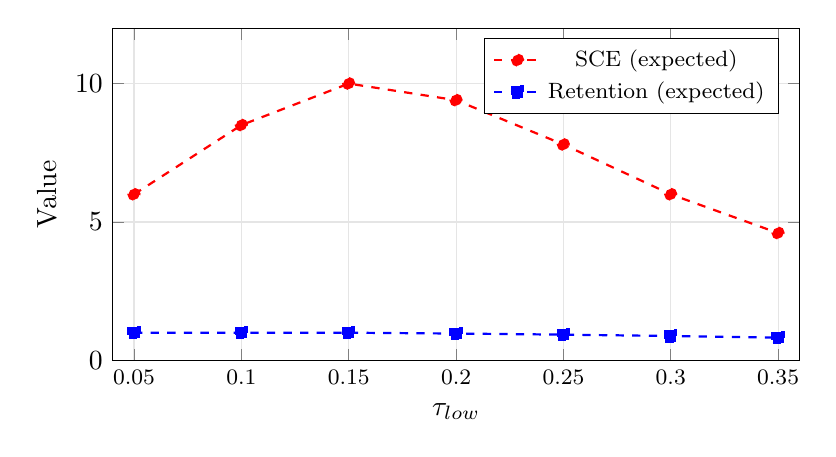
\begin{tikzpicture}
\begin{axis}[
  width=0.85\textwidth, height=5.8cm,
  xlabel={$\tau_{\text{low}}$}, ylabel={Value},
  xmin=0.04, xmax=0.36, ymin=0, ymax=12,
  xtick={0.05,0.10,0.15,0.20,0.25,0.30,0.35},
  xticklabel style={/pgf/number format/fixed, /pgf/number format/precision=2, font=\footnotesize},
  scaled x ticks=false,
  grid=both, grid style={gray!20},
  legend pos=north east, legend style={font=\footnotesize},
]
\addplot[red, thick, mark=*, dashed] coordinates
  {(0.05,6.0)(0.10,8.5)(0.15,10.0)(0.20,9.4)(0.25,7.8)(0.30,6.0)(0.35,4.6)};
\addlegendentry{SCE (expected)}
\addplot[blue, thick, mark=square*, dashed] coordinates
  {(0.05,1.00)(0.10,1.00)(0.15,1.000)(0.20,0.97)(0.25,0.93)(0.30,0.88)(0.35,0.82)};
\addlegendentry{Retention (expected)}
\end{axis}
\end{tikzpicture}
\caption[Expected threshold sweep]{Expected trend of sweeping
$\tau_{\text{low}}$ (dashed, to be populated from sweep runs). SCE is expected
to peak near the default while retention declines as more frames are cached.}
\label{fig:sweep}
\end{figure}

\section{Discussion}
\label{sec:exp-discussion}

The measured single-stream result demonstrates the behaviour the methodology
predicts: the fused-drift scheduler converts long quiescent intervals into
near-free cache reuse --- over $90\%$ of frames here --- while reserving full
reasoning for the rare genuine transitions, yielding an order-of-magnitude
reduction in VLM invocations at unit retention on this stream. Two caveats
frame this analysis. First, peak GPU memory is governed by the resident model
footprint rather than the policy, so the savings are in \emph{time and
energy}, not memory; per-run GPU instrumentation was not captured in this run
and is enabled for subsequent experiments. Second, the magnitude of every gain
depends on stream composition: this stream had limited semantic variation,
which inflates cache hit rate and retention, so the reported SCE is a
favourable-case figure. Establishing the full baseline comparison and the
ablation curves on identical frames --- and repeating the measurement across
streams of differing semantic density --- is the remaining empirical work.
